\section{LTI}
\label{tag:LTI}
ここではLTIについて述べさせてもらう\\
LTI(Learning Tools IterOperability)とは、IMS Global Learning Consortium(以下、IMTと呼ぶ)が、異なるプラットフォーム間(異なるLMS上)における学習支援ツールの相互運用を可能とする技術に関する企画を策定し、標準化した規格のことである。LTIに準拠することの具体的なイメージとして、次のようなケースを想定することができる。先代の研究によりできたNSFをツール・プロバイダとし、異なるLMSから利用するケース。(画像は後日作ってはります)\\


\begin{figure}[htbp]
  \begin{center}
    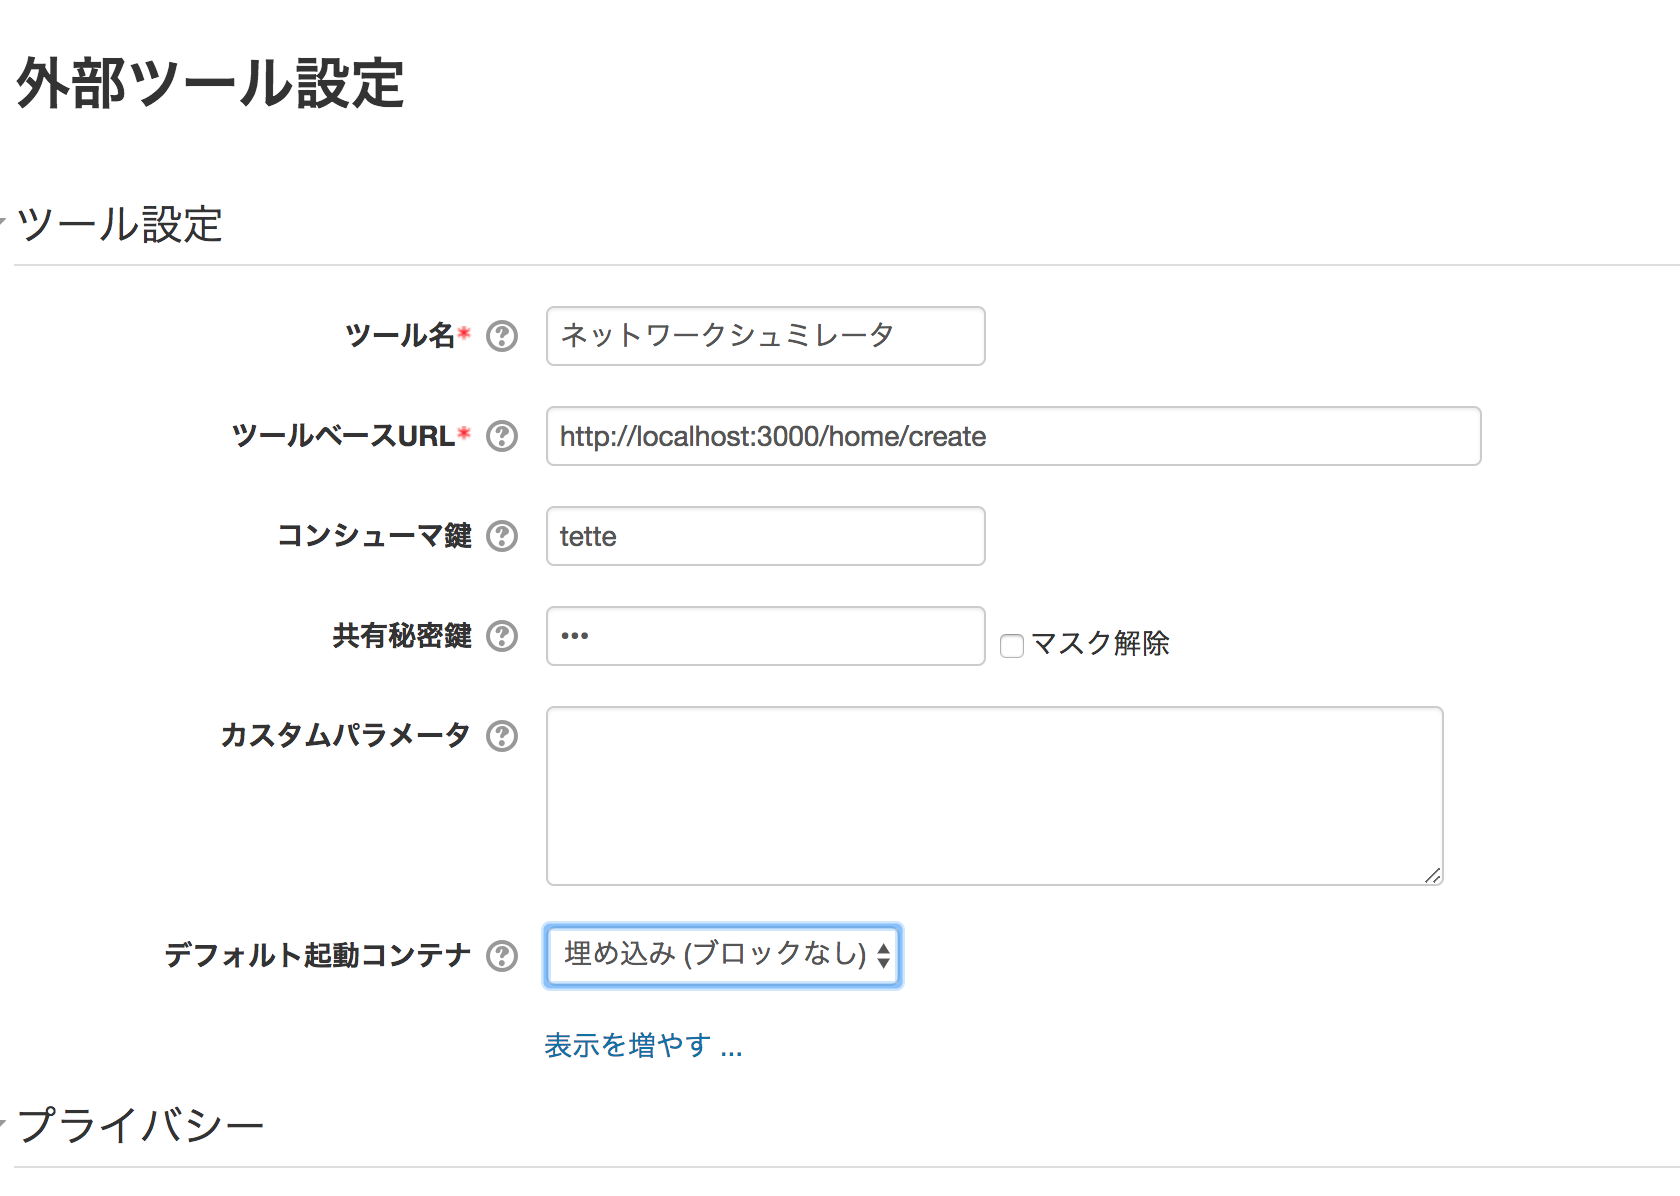
\includegraphics[clip,width=12.0cm,height=8.0cm]{img/moodleSet.png}
    \caption{moodle 外部ツール設定画面}
    \label{fig:moodle config}
  \end{center}
\end{figure}

\begin{figure}[htbp]
  \begin{center}
    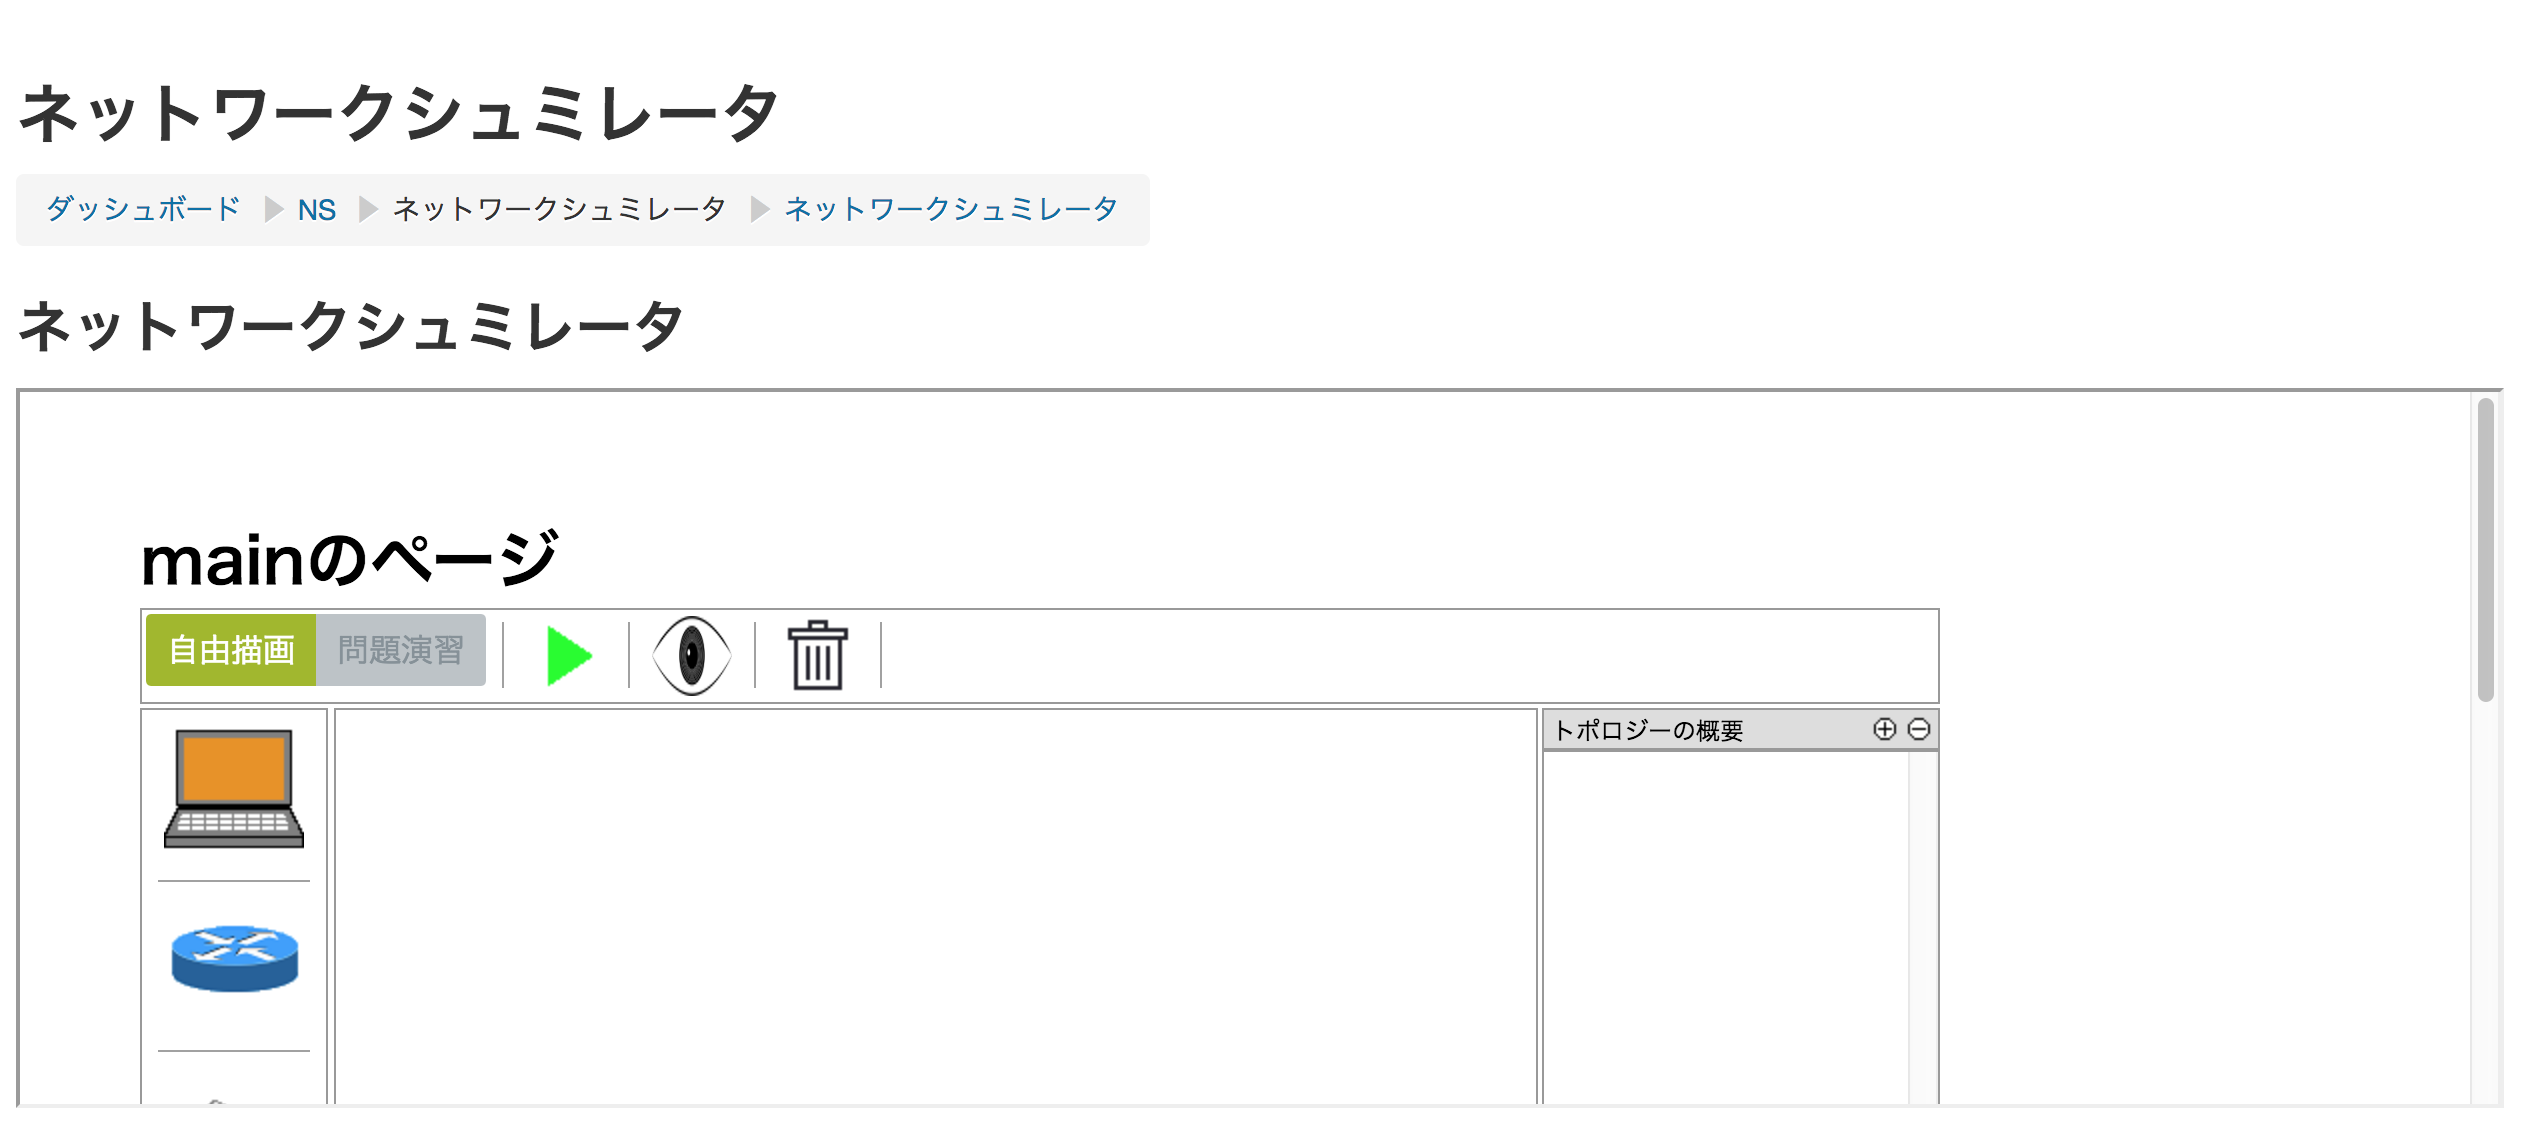
\includegraphics[clip,width=12.0cm,height=8.0cm]{img/LTIstart.png}
    \caption{moodle 外部ツール起動}
    \label{fig:moodle kidou}
  \end{center}
\end{figure}
